\subsection{Q2: Scaling with reference size} \label{SEEDsec:eval-refsize}

\begin{figure}[t]
  \begin{subfigure}{.5\textwidth}
    \centering
    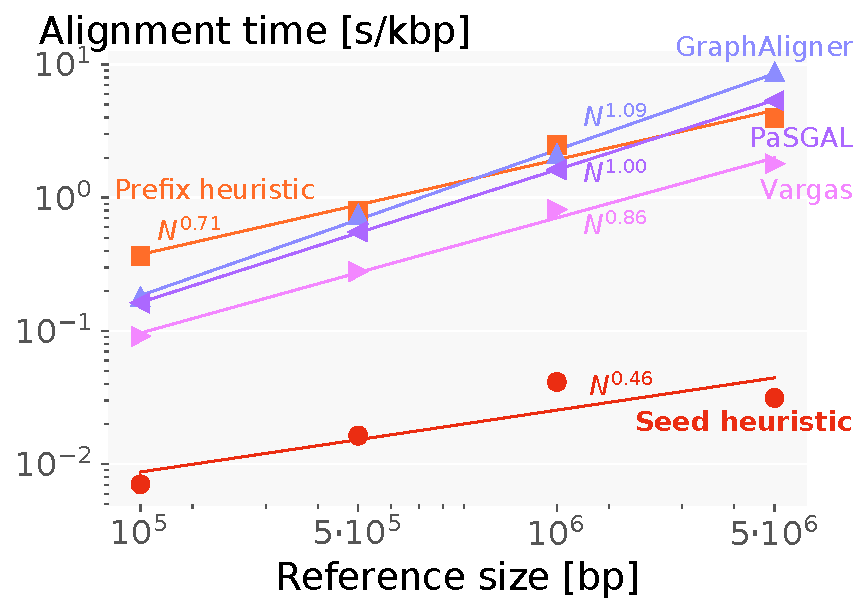
\includegraphics[width=\linewidth]{figures/illumina_spkb_vs_refsize-headxspkb.pdf}
  \end{subfigure}~\hspace{1em}
  \begin{subfigure}{.5\textwidth}
    \centering
    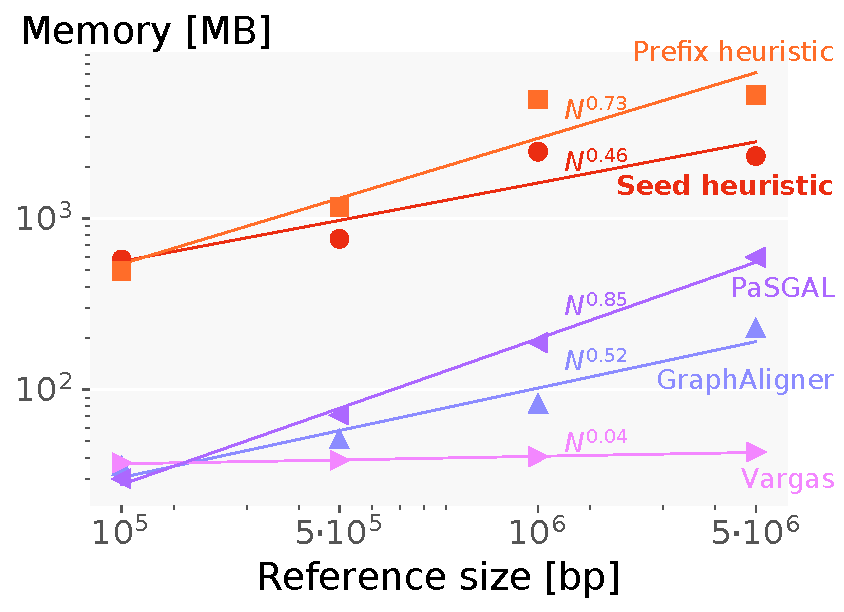
\includegraphics[width=\linewidth]{figures/illumina_memory_vs_refsize-headxmax_rss.pdf}
  \end{subfigure}~\hspace{1em} \caption[Performance scaling with reference size
  (short reads)]{Performance degradation with reference size for
  \textbf{Illumina reads}. Log-log plots of total alignment time (left) and
  memory usage (right) show the scaling difference between aligners.}
  \label{SEEDfig:illumina_scaling_with_genomesize}
\end{figure}

\begin{figure}[t]
  \begin{subfigure}{.5\textwidth}
    \centering
    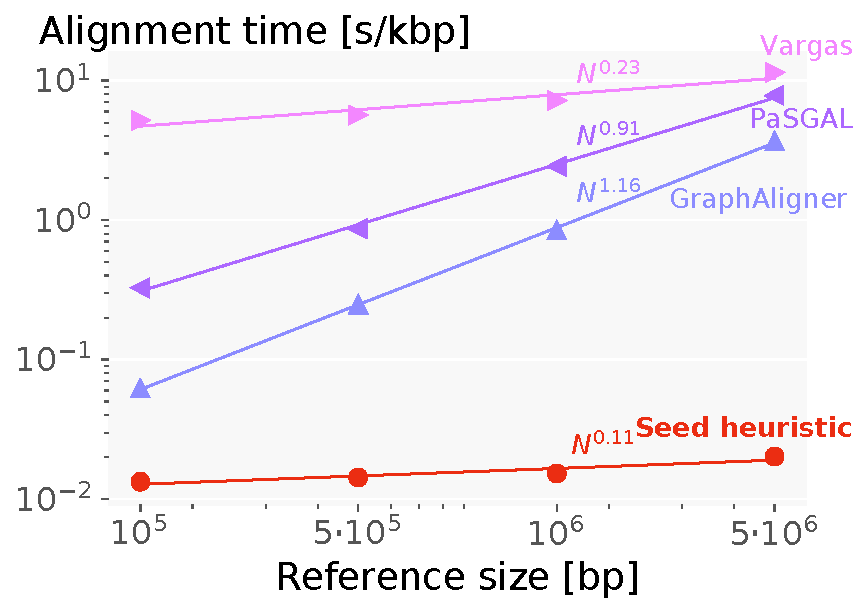
\includegraphics[width=\linewidth]{figures/hifi_spkb_vs_refsize-headxspkb.pdf}
  \end{subfigure}~\hspace{1em}
  \begin{subfigure}{.5\textwidth}
    \centering
    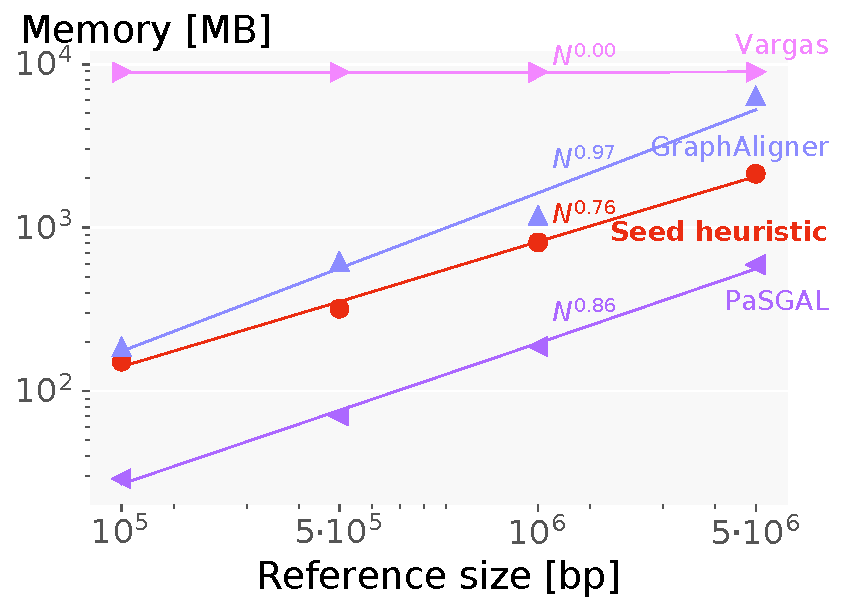
\includegraphics[width=\linewidth]{figures/hifi_memory_vs_refsize-headxmax_rss.pdf}
  \end{subfigure}~\hspace{1em} \caption[Performance scaling with reference size
  (long reads)]{Performance degradation with reference size for \textbf{HiFi
  reads}. Log-log plots of total alignment time (left) and memory usage (right)
  show the scaling difference between aligners. Linear best fits correspond to
  polynomials of varying degree.}
  \label{SEEDfig:hifi_scaling_with_genomesize}
\end{figure}

In order to study the scaling of the aligners in terms of the reference size, we
extracted prefixes of increasing length from MHC-linear. We then generated reads
from each prefix, and ran all tools on all prefixes with the corresponding
reads.

\para{Illumina reads}
\cref{SEEDfig:illumina_scaling_with_genomesize} shows the runtime scaling and memory
usage for Illumina reads. The \seedh was provided with 10k reads, while other
tools were provided with 1k reads.
%
The runtime of \graphaligner, \pasgal and \vargas grow approximately linearly
with the reference length, whereas the runtime of the \seedh grows roughly with
$\sqrt[2]{N}$, where $N$ is the reference size. Even on relatively small graphs
like MHC, the speedup of the \seedh reaches 200 times. Note that the scaling of
the \prefixh is substantially worse than the \seedh since the 200bp reads are
outside of its operational capabilities.

\para{HiFi reads}
\cref{SEEDfig:hifi_scaling_with_genomesize} shows the runtime scaling and memory
usage for HiFi reads. The respective total lengths of all aligned reads are 5Mbp
for the \seedh, 500kbp for \graphaligner, and 100kbp for \vargas and \pasgal. We
do not show the \prefixh, since it explores too many states and runs out of
memory.
%
Crucially, we observe that the runtime of the \seedh is almost independent of
the reference size, growing as $N^{0.11}$. We believe this improved trend
compared to short reads is because the \seedh obtains better guidance on long
reads, as it can leverage information from the whole read.

For both Illumina and HiFi reads, we observe near-linear scaling for \pasgal and
\graphaligner as expected from the theoretical $\Oh(Nm)$ runtime of the DP
approaches. We conjecture that the runtime of \vargas for long reads is
dominated by the dependence from the read length, which is why on HiFi reads we
observe better than linear runtime dependency on $N$ but very large runtime. The
current alignment bottleneck of \astarixseeds is its memory usage, which is
distributed between remembering crumbs and holding a queue of explored states.